% SALSA overview figures — ONE source, TWO rendered SVGs.
%
% `render.sh` compiles this to a 2-page PDF (the `standalone` class crops each
% tikzpicture to its own page) and exports:
%     page 1  ->  salsa_system.svg   (embedded as Figure 1 in ../salsa.md)
%     page 2  ->  salsa_tile.svg     (embedded as Figure 2 in ../salsa.md)
%
% To use: paste the two figures from the SALSA paper into the marked tikzpicture
% bodies below, and copy whatever \usetikzlibrary / \definecolor / \newcommand
% lines the paper preamble used into the PREAMBLE block. Then: `bash render.sh`.

% `dvipsnames` defines Orchid / BlueViolet / DarkOrchid (the paper's colors).
% Queue it before standalone[tikz] loads xcolor, else xcolor is already loaded
% without the option and the names are undefined.
\PassOptionsToPackage{dvipsnames}{xcolor}
\documentclass[tikz,border=4pt]{standalone}
\usepackage{tikz}
\usetikzlibrary{chains,arrows,arrows.meta,calc,positioning}
\usepackage{xcolor}
\usetikzlibrary{arrows.meta,positioning,calc,fit,backgrounds,shapes.geometric}
\usetikzlibrary{angles,quotes,positioning,calc,shapes.geometric, arrows.meta, shadows.blur}
\usetikzlibrary{decorations.pathreplacing}  % brace decorations (\draw[decorate, decoration={brace}])

\newcommand{\subsf}{\sf \scriptscriptstyle}
\newcommand{\bs}{\boldsymbol}
\newcommand{\mc}{\mathcal}
\newcommand{\wh}{\widehat}
\newcommand{\ov}{\overline}

% ---- PREAMBLE: paste the paper's libraries / colors / macros here ----------
% \definecolor{salsapurple}{RGB}{...}
% \newcommand{\foo}{...}
% ---------------------------------------------------------------------------

\begin{document}

%% ========= Figure 1 — SALSA system  ( -> salsa_system.svg ) =========
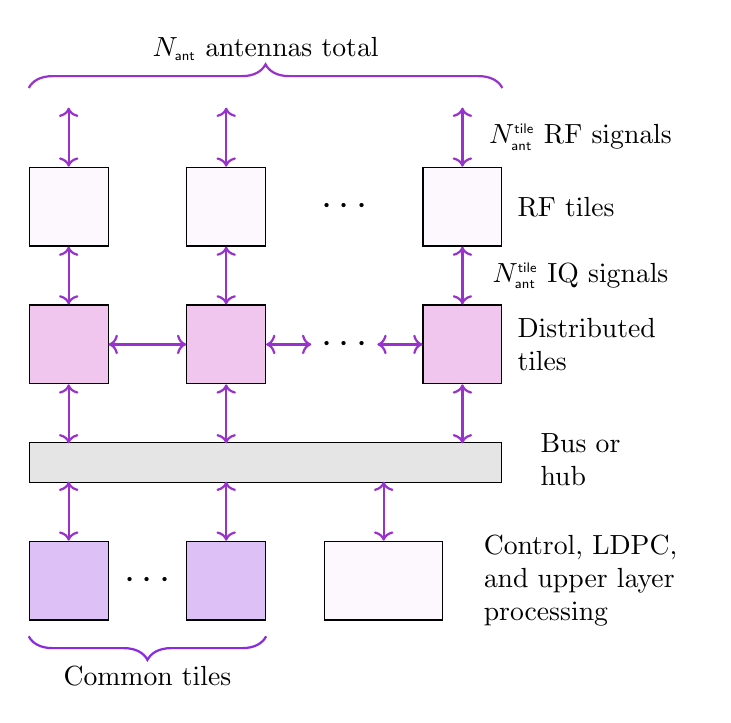
\begin{tikzpicture}
  % Styles
  \tikzstyle{tile} = [rectangle, draw, minimum height=1cm, minimum width=1cm, text centered]
  \tikzstyle{rffetile} = [tile,fill=Orchid!5]
  \tikzstyle{disttile} = [tile,fill=Orchid!40]
  \tikzstyle{comtile} = [tile,fill=BlueViolet!30]
  \tikzstyle{bus} = [text centered]
  \tikzstyle{arrow} = [draw, -latex]
  \tikzstyle{connection} = [<->, thick, DarkOrchid]

  % Nodes
  % RF tiles
  \node[rffetile] (rffe1) {};
  \node[rffetile, right of=rffe1, xshift=1cm] (rffe2) {};
  \node[right of=rffe2, xshift=0.5cm] (rffedots) {\Large $\cdots$};
  \node[rffetile, right of=rffedots, xshift=0.5cm] (rffe3) {};
  \node[right of=rffe3, xshift=0.7cm] {\parbox{2cm}{RF tiles}};

  % Distributed tiles
  \node[disttile, below of=rffe1,
  yshift=-0.75cm] (dist1) {};
  \node[disttile, right of=dist1, xshift=1cm] (dist2) {};
  \node[right of=dist2, xshift=0.5cm] (distdots) {\Large $\cdots$};
  \node[disttile, right of=distdots, xshift=0.5cm] (dist3) {};
  \node[right of=dist3,
  xshift=0.7cm] {\parbox{2cm}{Distributed\\tiles}};
 
  
  % Bus 
  \node[rectangle, draw, fill=gray!20, minimum width=6cm, minimum height=0.5cm, below of=dist2, xshift=0.5cm, yshift=-0.5cm] (bus) {};
  \node[right of=bus, xshift=3cm] {\begin{tabular}{l}Bus or\\ hub
  \end{tabular}};

  % Common tiles
  \node[comtile, below of=dist1,
  yshift=-2cm] (com1) {};
  \node[right of=com1, xshift=0cm] (comdots) {\Large $\cdots$};
  \node[comtile, right of=comdots,
  xshift=0cm] (com2) {};
  
  \draw[decorate, thick, BlueViolet, decoration={brace, mirror,amplitude=0.3cm}] ([yshift=-0.2cm] com1.south west) -- ([yshift=-0.2cm] com2.south east) node[midway] (brace) {};

  \node[below of=brace,yshift=0.5cm] {Common tiles};

  % Upper layer processing
  \node[rffetile, right of=com2,
  minimum width=1.5cm, xshift=1cm] (upper) {};
  \node [right of=upper,xshift=1.5cm] {\begin{tabular}{l}Control, LDPC,\\
  and upper layer\\ processing
  \end{tabular}}; 

  % Draw arrows
  \foreach \i in {1,2,3} {
    \draw[connection] (rffe\i.south) -- (dist\i.north) node [midway] (distcon\i) {};
    \draw[connection] (dist\i.south) -- ++ (0,-0.75);
    \draw[connection] (rffe\i.north) -- ++(0,0.75) node [midway] (rffecon\i) {};
  };
  \draw[connection] (com1.north) -- ++(0,0.75);
  \draw[connection] (com2.north) -- ++(0,0.75);
  \draw[connection] (upper.north) -- ++(0,0.75);
  \draw[connection] (dist1) -- (dist2);
  \draw[connection] (dist2) -- (distdots);
  \draw[connection] (dist3) -- (distdots);

  \node[right of=rffecon3, xshift=0.5cm] {\begin{tabular}{l}$N^{\subsf tile}_{\subsf ant}$ RF signals
  \end{tabular}};
  \node[right of=distcon3, xshift=0.5cm] {\begin{tabular}{l}$N^{\subsf tile}_{\subsf ant}$ IQ signals
  \end{tabular}};

  \draw[decorate, thick, DarkOrchid, decoration={brace, amplitude=0.3cm}] ([yshift=1cm] rffe1.north west) -- ([yshift=1cm] rffe3.north east) node[midway] (rffe_brace) {};
  \node [above of=rffe_brace,yshift=-0.5cm] {$N_{\subsf ant}$ antennas total};
  
\end{tikzpicture}

%% ========= Figure 2 — distributed tile  ( -> salsa_tile.svg ) =========
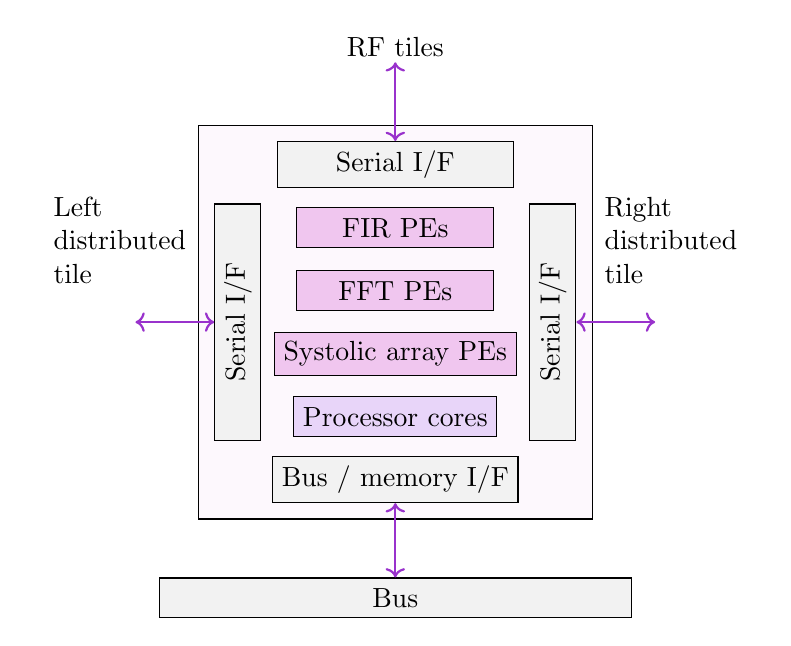
\begin{tikzpicture}

   % Styles
  \tikzstyle{blk} = [rectangle, draw, minimum height=0.5cm, minimum width=1cm, text centered]
  \tikzstyle{peblk} = [blk,fill=Orchid!40,
  minimum height=0.5cm, minimum width=2.5cm]
  \tikzstyle{procblk} = [blk,minimum height=0.5cm, minimum width=2.5cm,fill=BlueViolet!20]
  \tikzstyle{ifblk} = [blk,fill=gray!10]
  \tikzstyle{connection} = [<->, thick, DarkOrchid]

  % background
  \node[blk,fill=Orchid!5,minimum height=5cm, minimum width=5cm] at (0,0) {};

  % Antenna IF
  \node[ifblk, minimum width=3cm] at (0,2) (antif) {Serial I/F};
  \draw[connection] (antif.north) -- ++(0,1)
    node[above] (antiftext) {};
  \node[above of=antif,yshift=0.5cm] {RF tiles};

  % Distributed serial I/F to the left
  \node[ifblk, minimum width=3cm,rotate=90] at (-2,0) (distifleft) {Serial I/F};
  \draw[connection] (distifleft.north) -- ++(-1,0);
  \node[left of=distifleft,xshift=-0.5cm,yshift=1cm]
    {\begin{tabular}{l} Left\\distributed\\tile \end{tabular} };

  % Distributed serial I/F to the right
  \node[ifblk, minimum width=3cm,rotate=90] at (2,0) (distifright) {Serial I/F};
  \draw[connection] (distifright.south) -- ++(1,0);
  \node[right of=distifright,xshift=0.5cm,yshift=1cm]
    {\begin{tabular}{l} Right\\distributed\\tile \end{tabular} };

  % Processing units
  \node[peblk] at (0,1.2) (fir) {FIR PEs};
  \node[peblk, below of=fir,yshift=0.2cm] (fft) {FFT PEs};
  \node[peblk, below of=fft,yshift=0.2cm] (array) {Systolic array PEs};
  \node[procblk, below of=array,yshift=0.2cm] (proc) {Processor cores};

  % Bus interface
  \node[ifblk, minimum width=3cm] at (0,-2) (busif) {Bus / memory I/F};
  \node[ifblk, minimum width=6cm,below of=busif,
  yshift=-0.5cm] (bus) {Bus};
  
  \draw[connection] (busif.south) -- (bus.north);
\end{tikzpicture}

\end{document}
